\documentclass{article}
\usepackage[utf8]{inputenc}
\usepackage{amsmath}
\usepackage{amsfonts}
\usepackage{amssymb}
\usepackage{graphicx}

\title{Efficient Models for Large Datasets using glmmTMB with Xr Terms}
\author{Erlend Myhre /& Håvard Kolve}
\date{\today}

\begin{document}

\maketitle

\section{Introduction}
The aim of this project is to implement computationally efficient models for analyzing large datasets using the \texttt{glmmTMB} package with Xr terms. The Xr terms are matrices of basis functions that are parameterized as random effects through \texttt{mgcv::smooth2random} and constructed using \texttt{mgcv::smoothCon}.

\section{Efficiency of Xr Terms}
\begin{itemize}
    \item Xr terms are computationally efficient, both in terms of speed and memory usage.
    \item The number of knots (basis functions) is kept low to enhance efficiency.
    \item Limiting the number of knots also acts as an implicit regularization method to prevent overfitting.
    \item Choosing less flexible spline types like cubic regression splines (\texttt{bs="cr"}) further prevents overfitting by generating smoother curves.
\end{itemize}

\section{Empirical Observations}
Based on empirical data and tests, explicit penalization or regularization may not be necessary when the method is applied correctly on large and complex datasets.

\section{Computationally Efficient Generation}
Smooth terms can be generated efficiently due to the low value of \(k\) and the efficient construction of cubic regression splines.

\section{Parallelization}
\begin{itemize}
    \item The method can be further accelerated by parallelizing the smooth term generation.
    \item Model fitting can also be done in parallel using futures or similar techniques.
    \item The same parallelization can be applied during the training and validation evaluations.
\end{itemize}

\section{Hypothesis and Goals}
The primary hypothesis is that efficient models for large datasets can be developed using custom-fitted flexible (but not overly so) predictors in the form of Xr terms. This method is expected to be both faster and more resource-efficient than current complex models like spline regression models (GAMs etc.).

\section{Practical Implications}
\begin{itemize}
    \item Resource saving: Reduces computational time and memory requirements.
    \item Cost-effective: Lowers the cost associated with cloud-based services or local hardware investments.
    \item These models are intended for use by competent users and can fit complex, nonlinear data at a reduced computational cost.
\end{itemize}

\section{Conclusions}
The method offers a promising way to analyze large datasets efficiently while maintaining model accuracy and flexibility. Further automation of the process is straightforward and presents an excellent avenue for future work.


\subsection{Visuals}

\section{Learning Curves}

\begin{figure}[h]
    \centering
    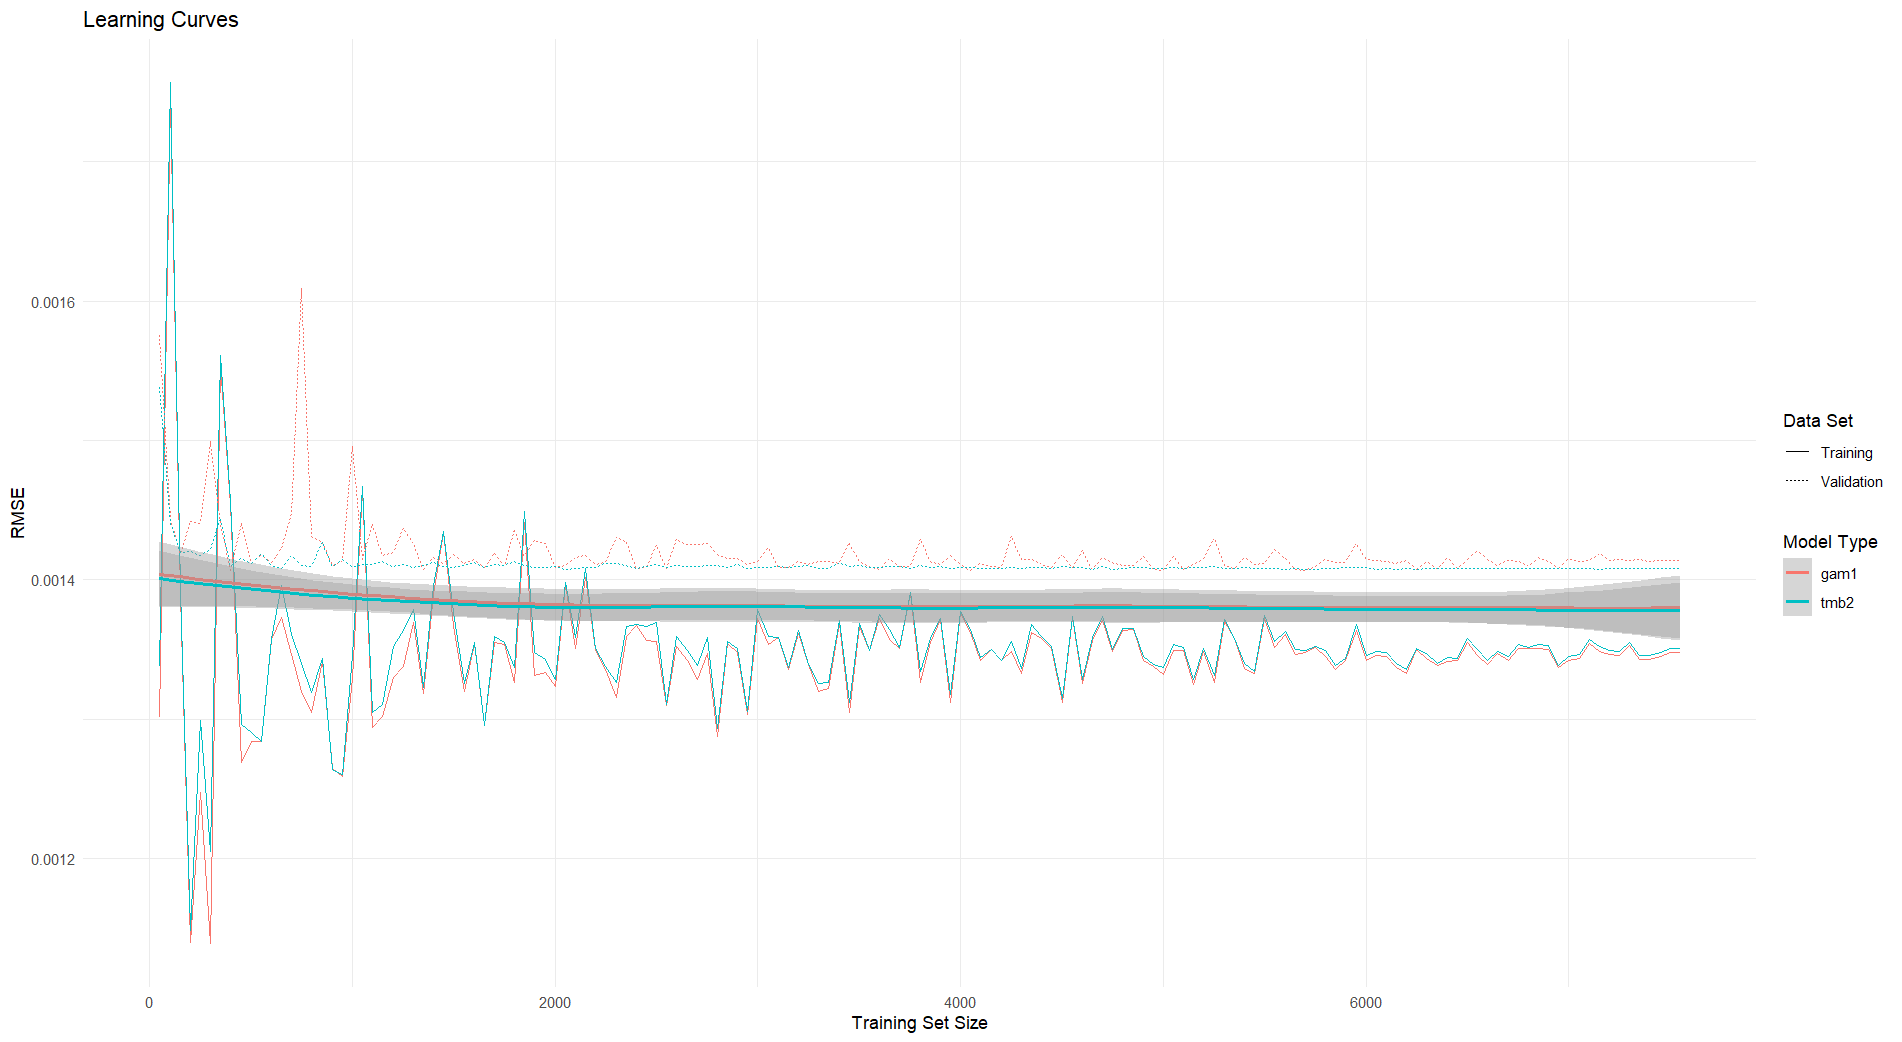
\includegraphics[width=0.9\linewidth]{visuals/Learning_curves_aapl.png}
    \caption{Learning Curve for AAPL}
\end{figure}

\begin{figure}[h]
    \centering
    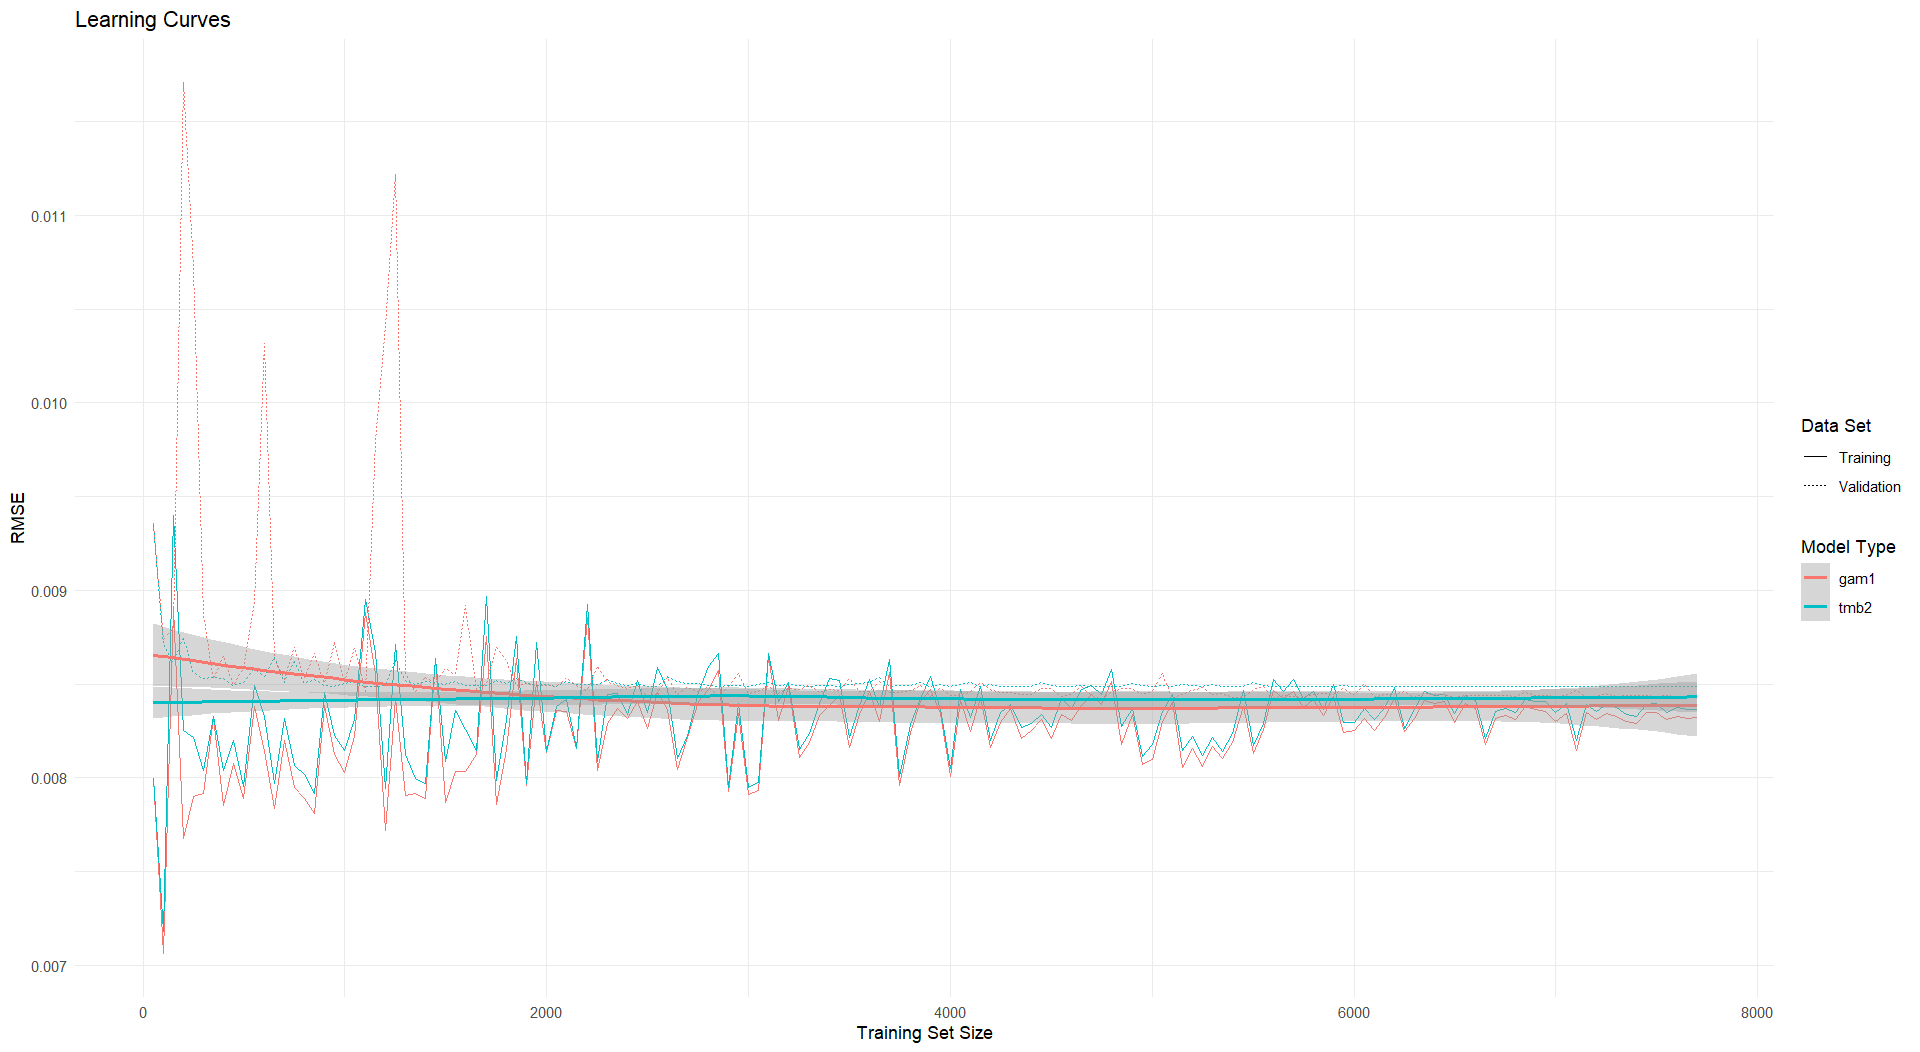
\includegraphics[width=0.9\linewidth]{visuals/Learning_curves_ko.png}
    \caption{Learning Curve for KO}
\end{figure}

\begin{figure}[h]
    \centering
    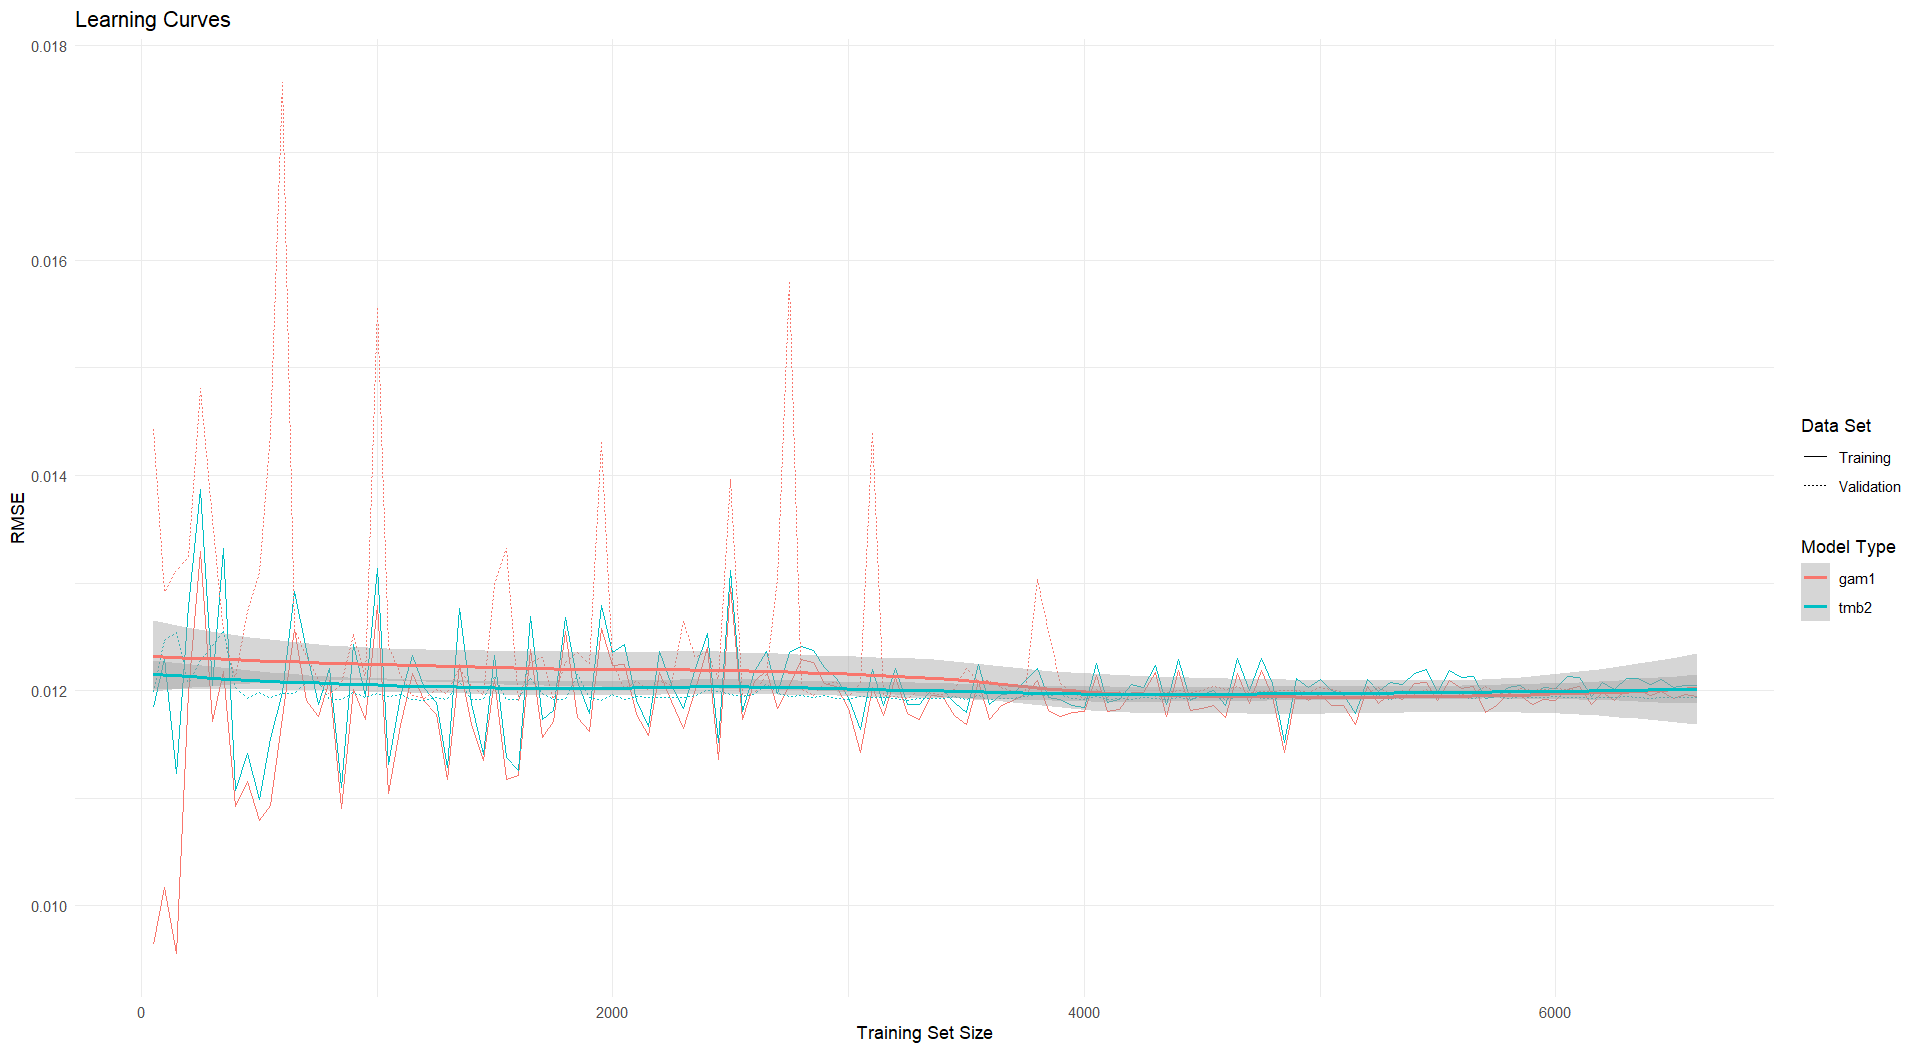
\includegraphics[width=0.9\linewidth]{visuals/Learning_curves_msft.png}
    \caption{Learning Curve for MSFT}
\end{figure}

\begin{figure}[h]
    \centering
    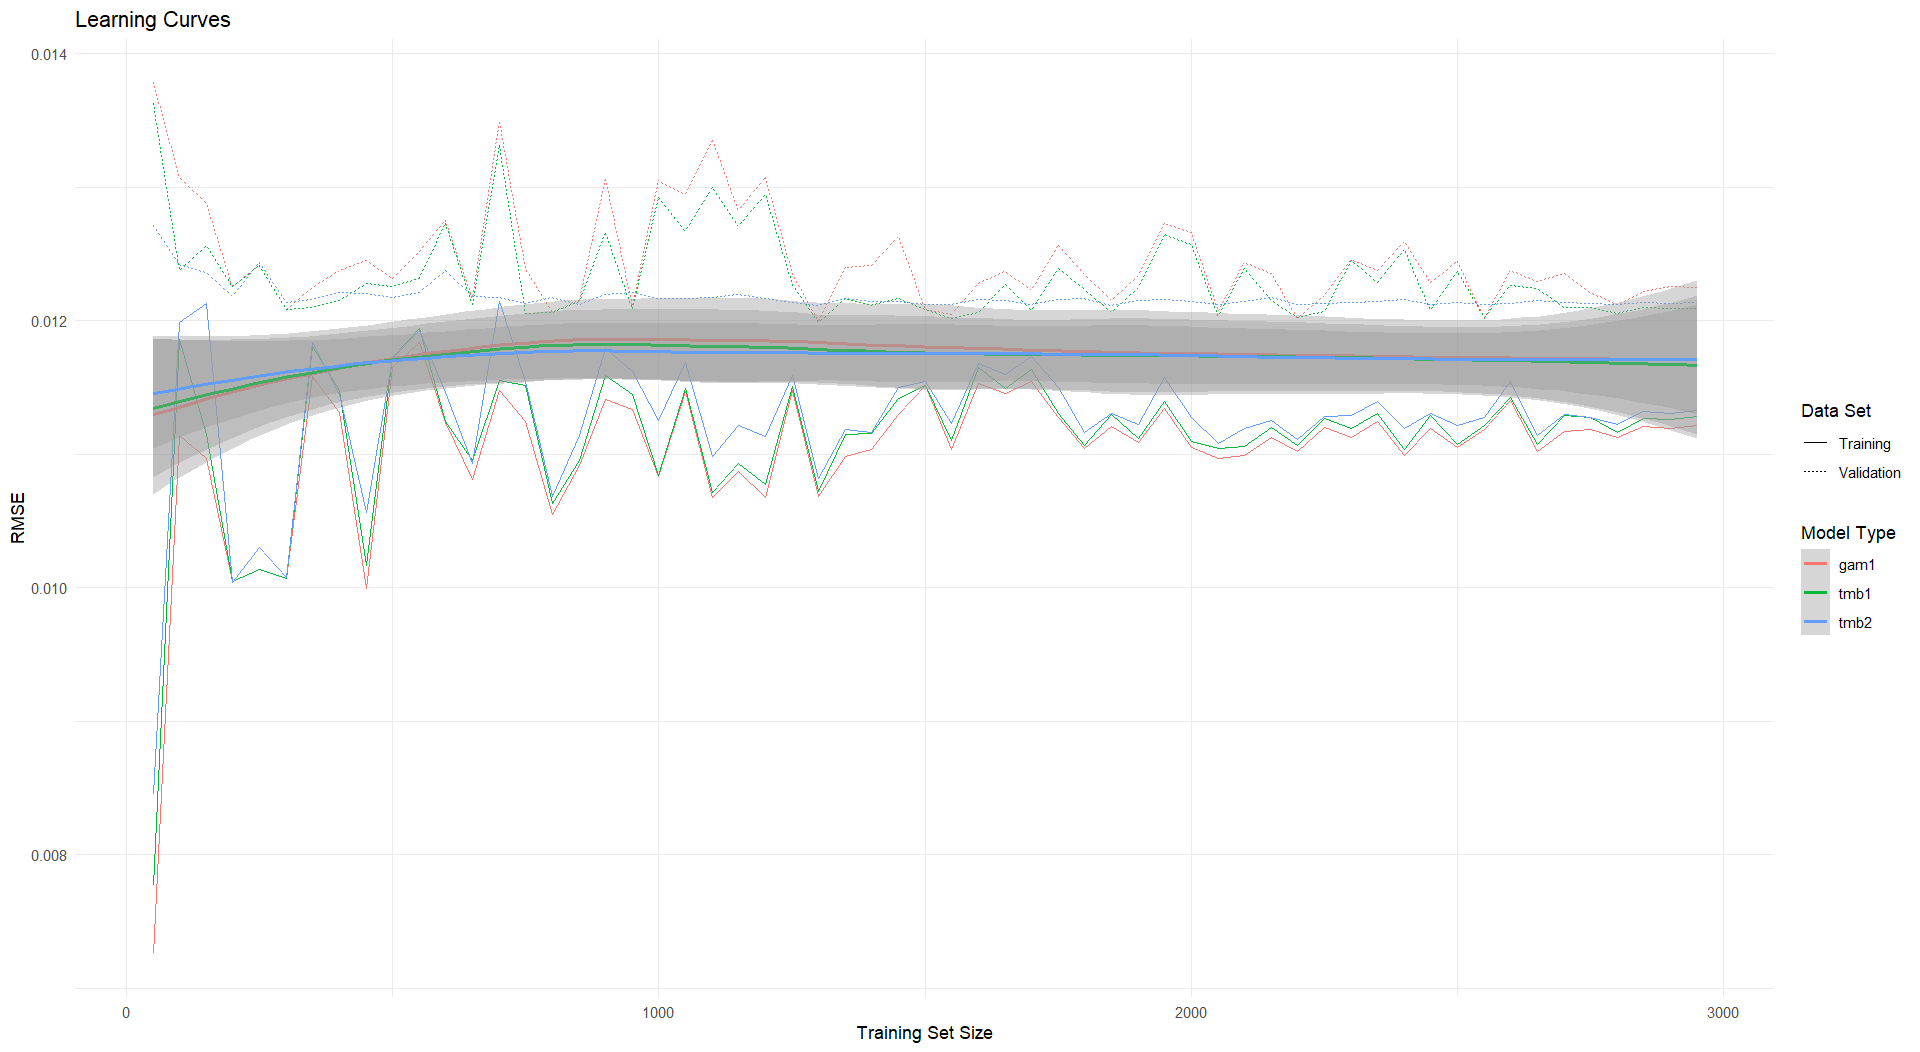
\includegraphics[width=0.9\linewidth]{visuals/Learning_curves_nvda.png}
    \caption{Learning Curve for NVDA}
\end{figure}

\begin{figure}[h]
    \centering
    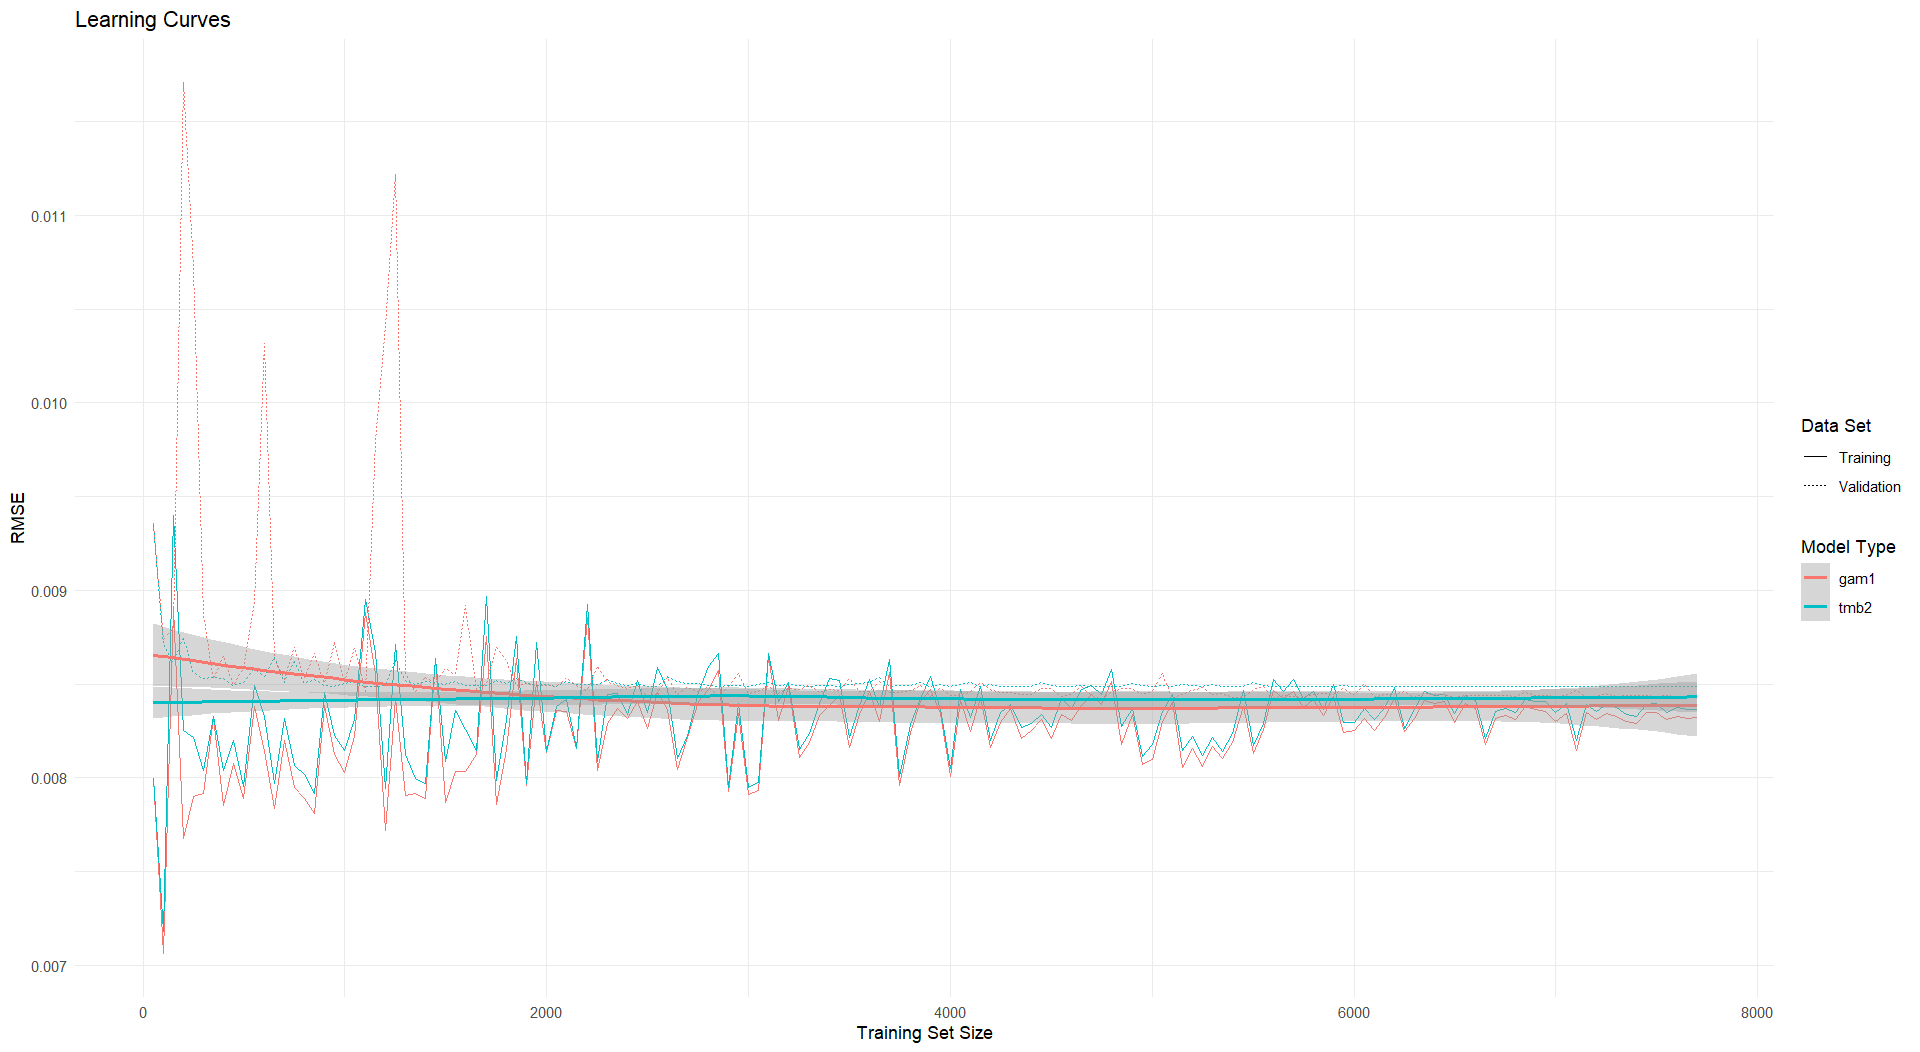
\includegraphics[width=0.9\linewidth]{visuals/Learning_curves_snow.png}
    \caption{Learning Curve for SNOW}
\end{figure}

\subsection{Prediction vs Observation}

\begin{figure}[h]
    \centering
    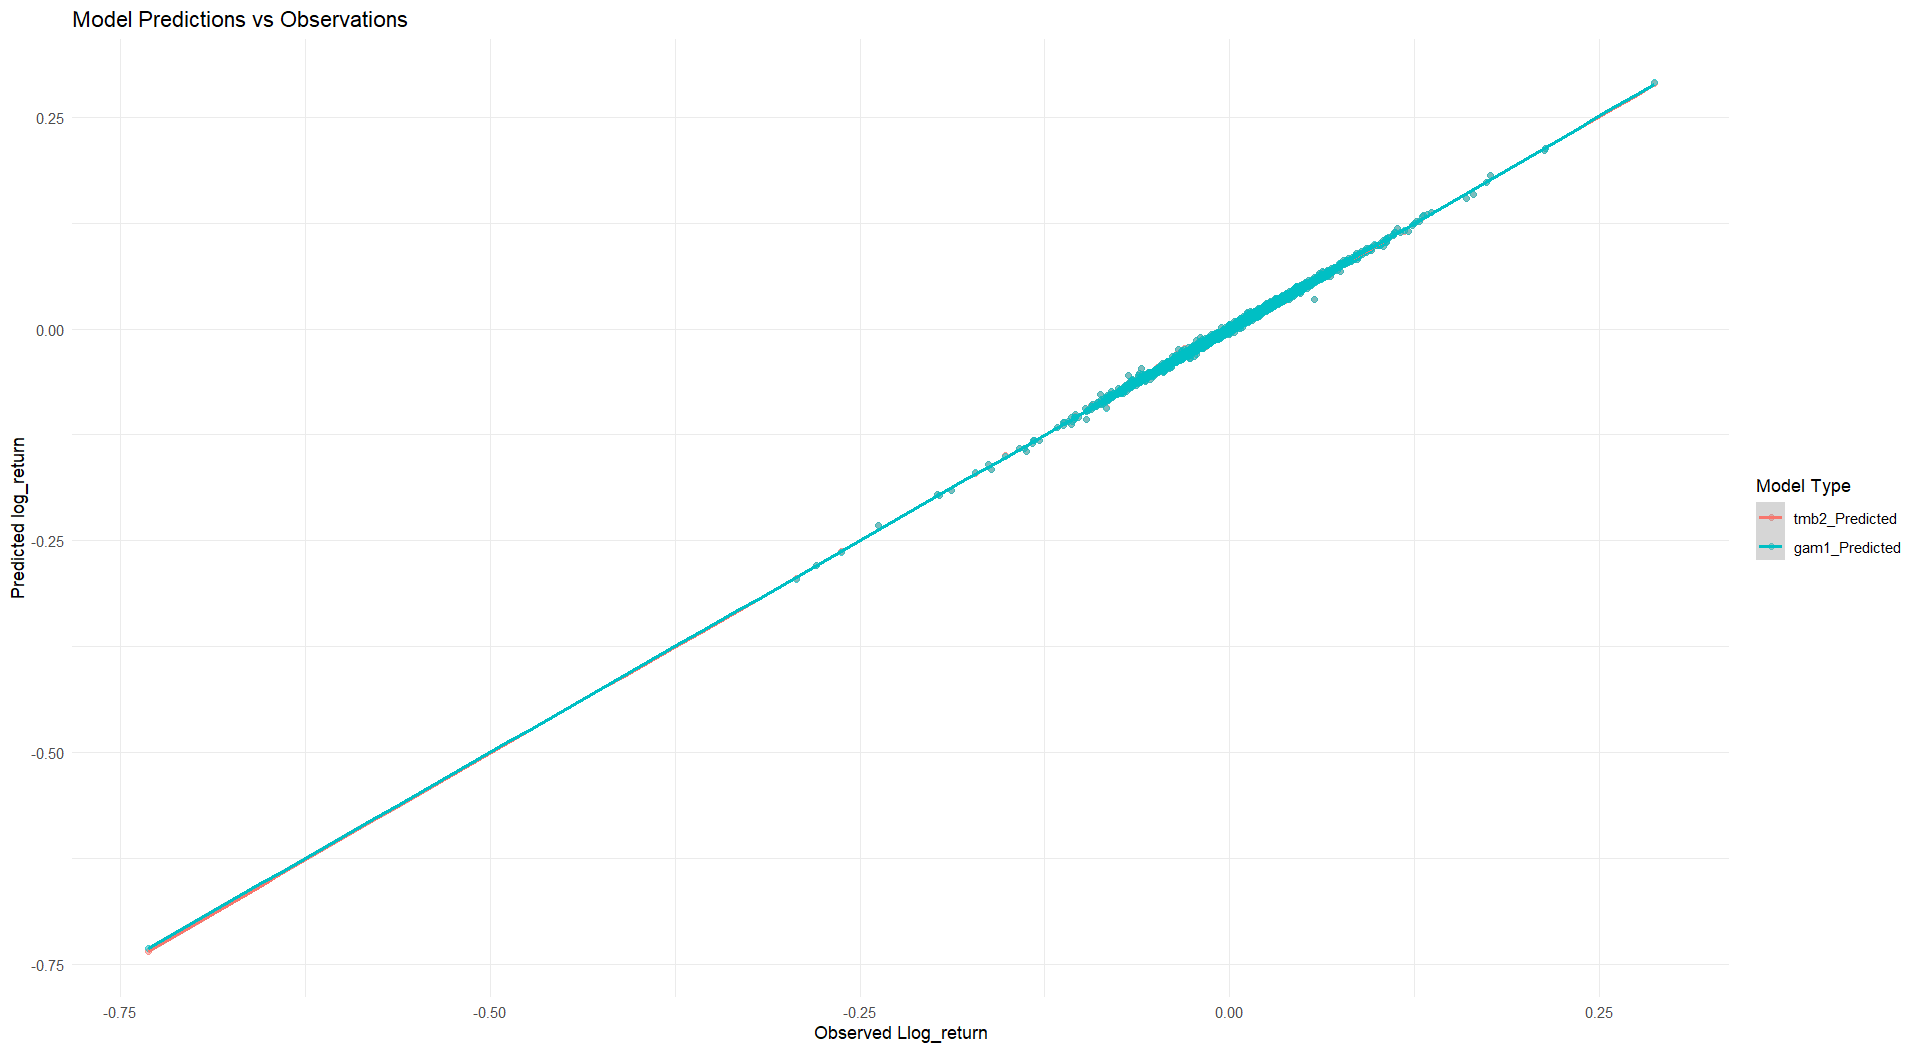
\includegraphics[width=0.9\linewidth]{visuals/pred_obs_aapl.png}
    \caption{Prediction vs Observation for AAPL}
\end{figure}

\begin{figure}[h]
    \centering
    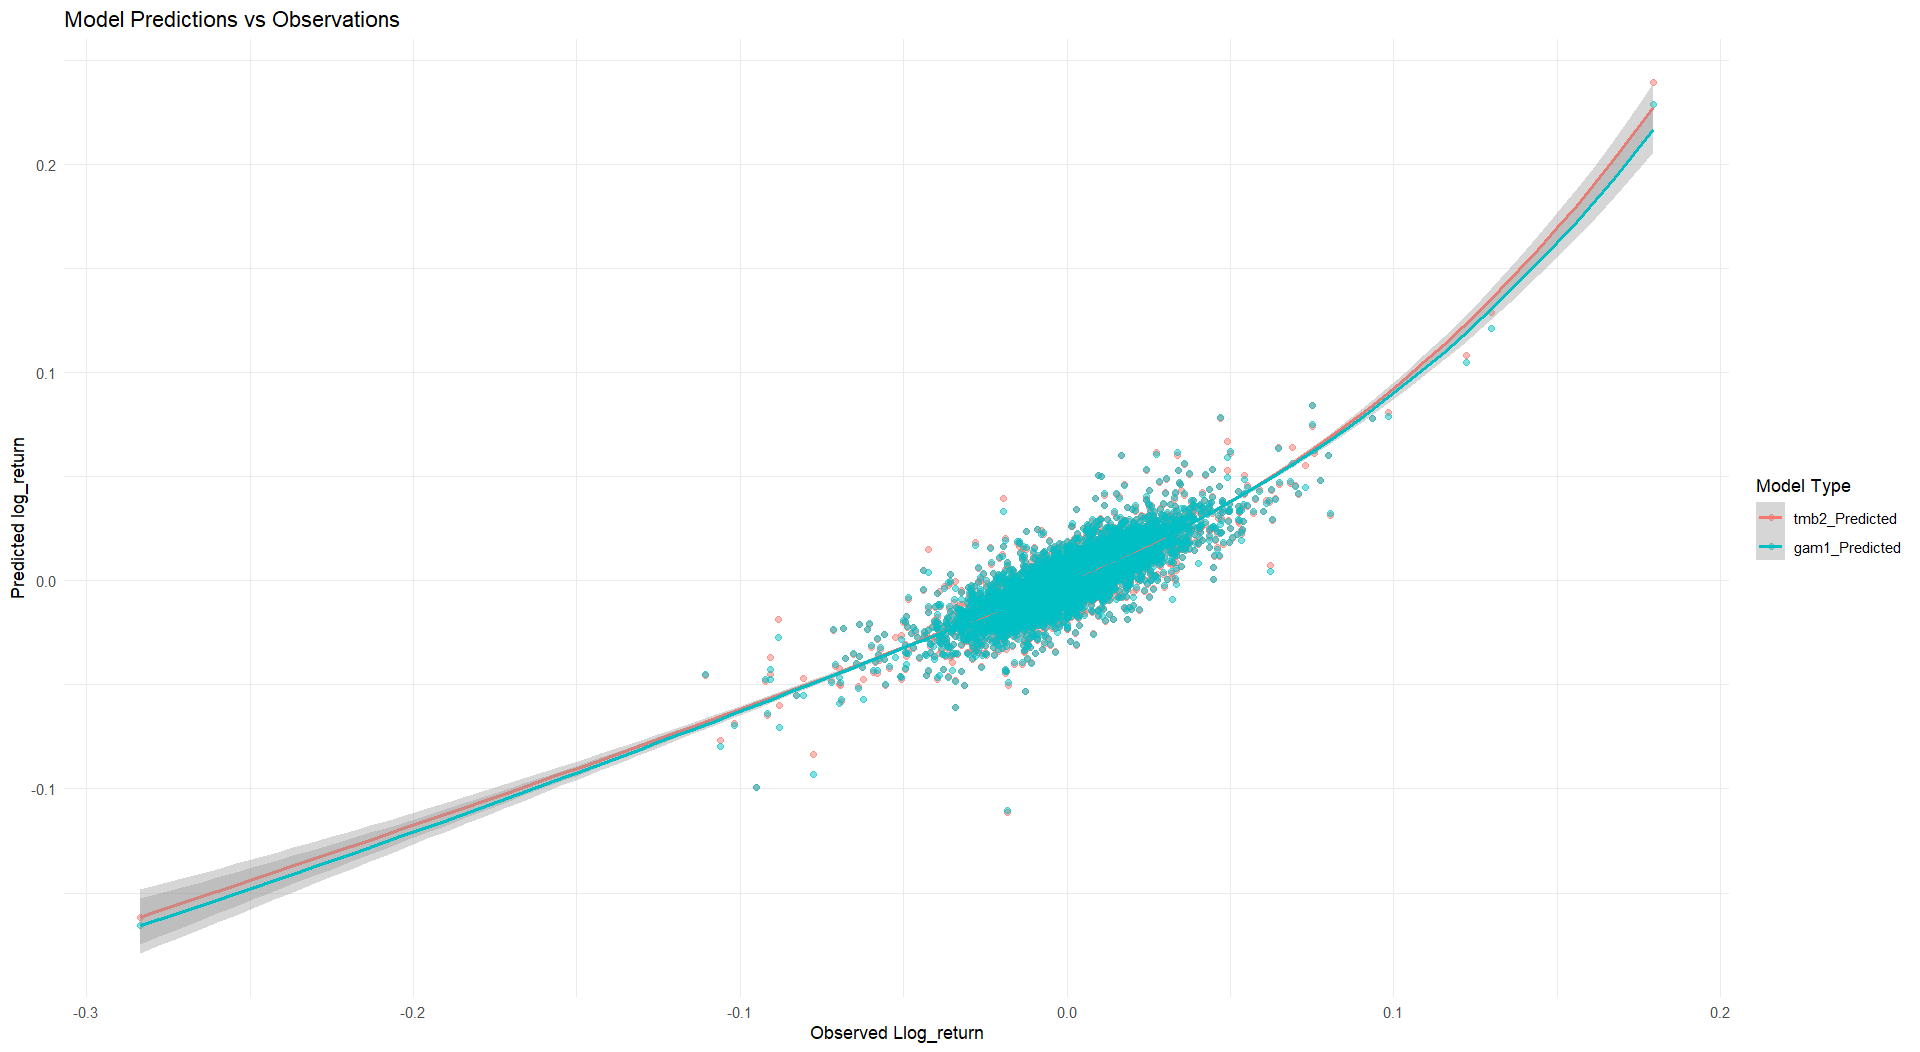
\includegraphics[width=0.9\linewidth]{visuals/pred_obs_ko.png}
    \caption{Prediction vs Observation for KO}
\end{figure}

\begin{figure}[h]
    \centering
    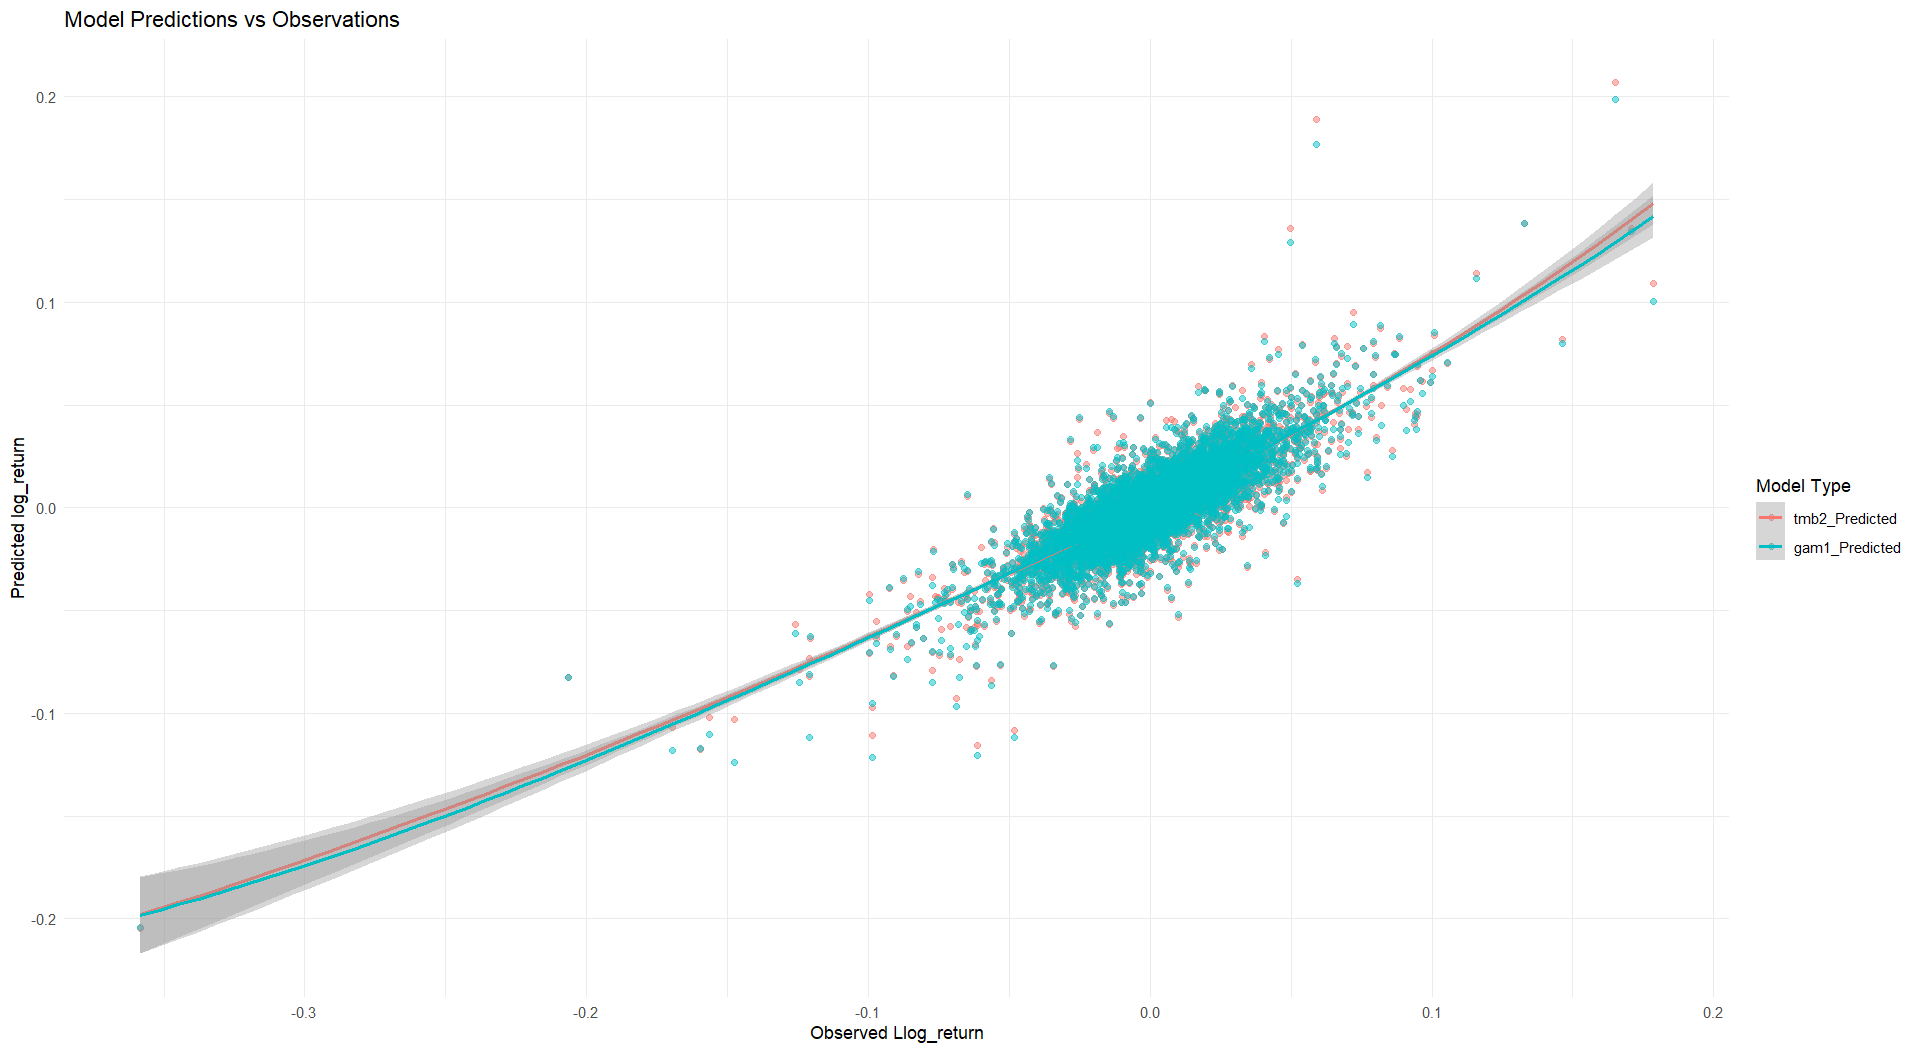
\includegraphics[width=0.9\linewidth]{visuals/pred_obs_msft.png}
    \caption{Prediction vs Observation for MSFT}
\end{figure}

\begin{figure}[h]
    \centering
    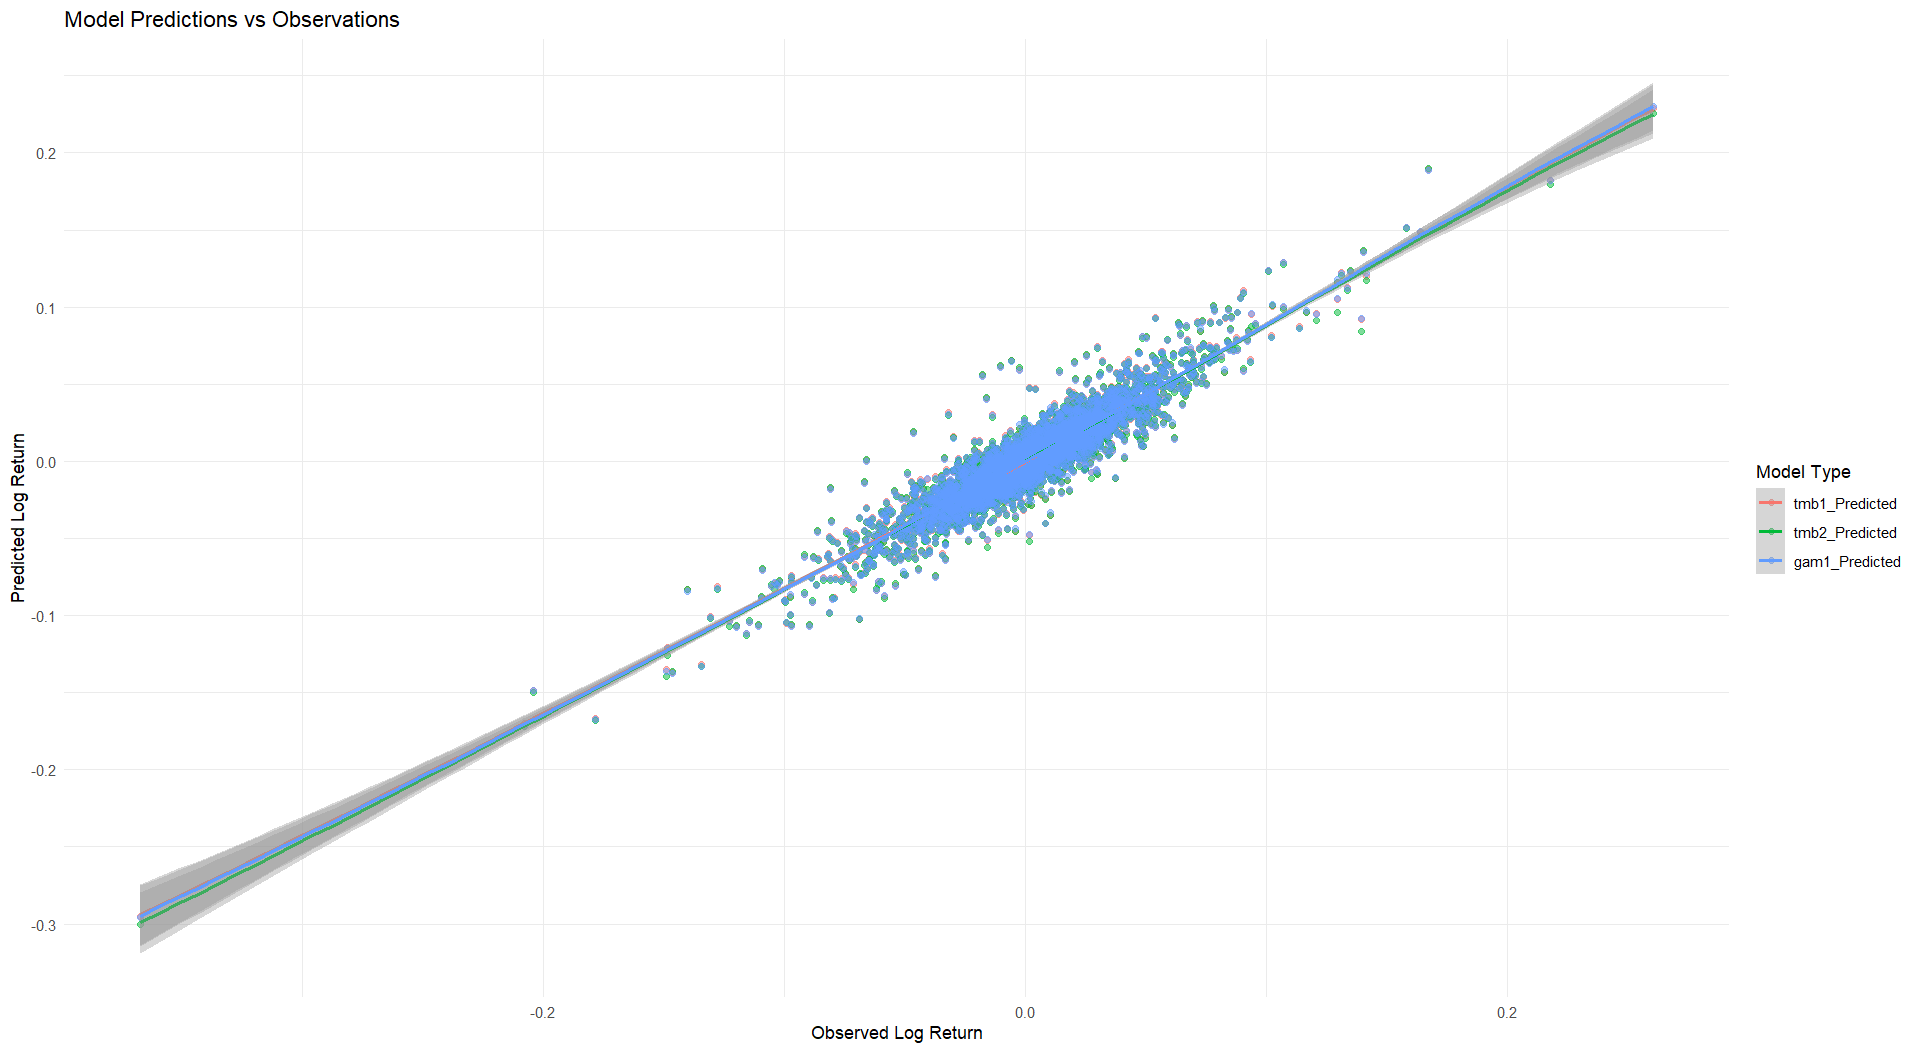
\includegraphics[width=0.9\linewidth]{visuals/pred_obs_nvda.png}
    \caption{Prediction vs Observation for NVDA}
\end{figure}

\begin{figure}[h]
    \centering
    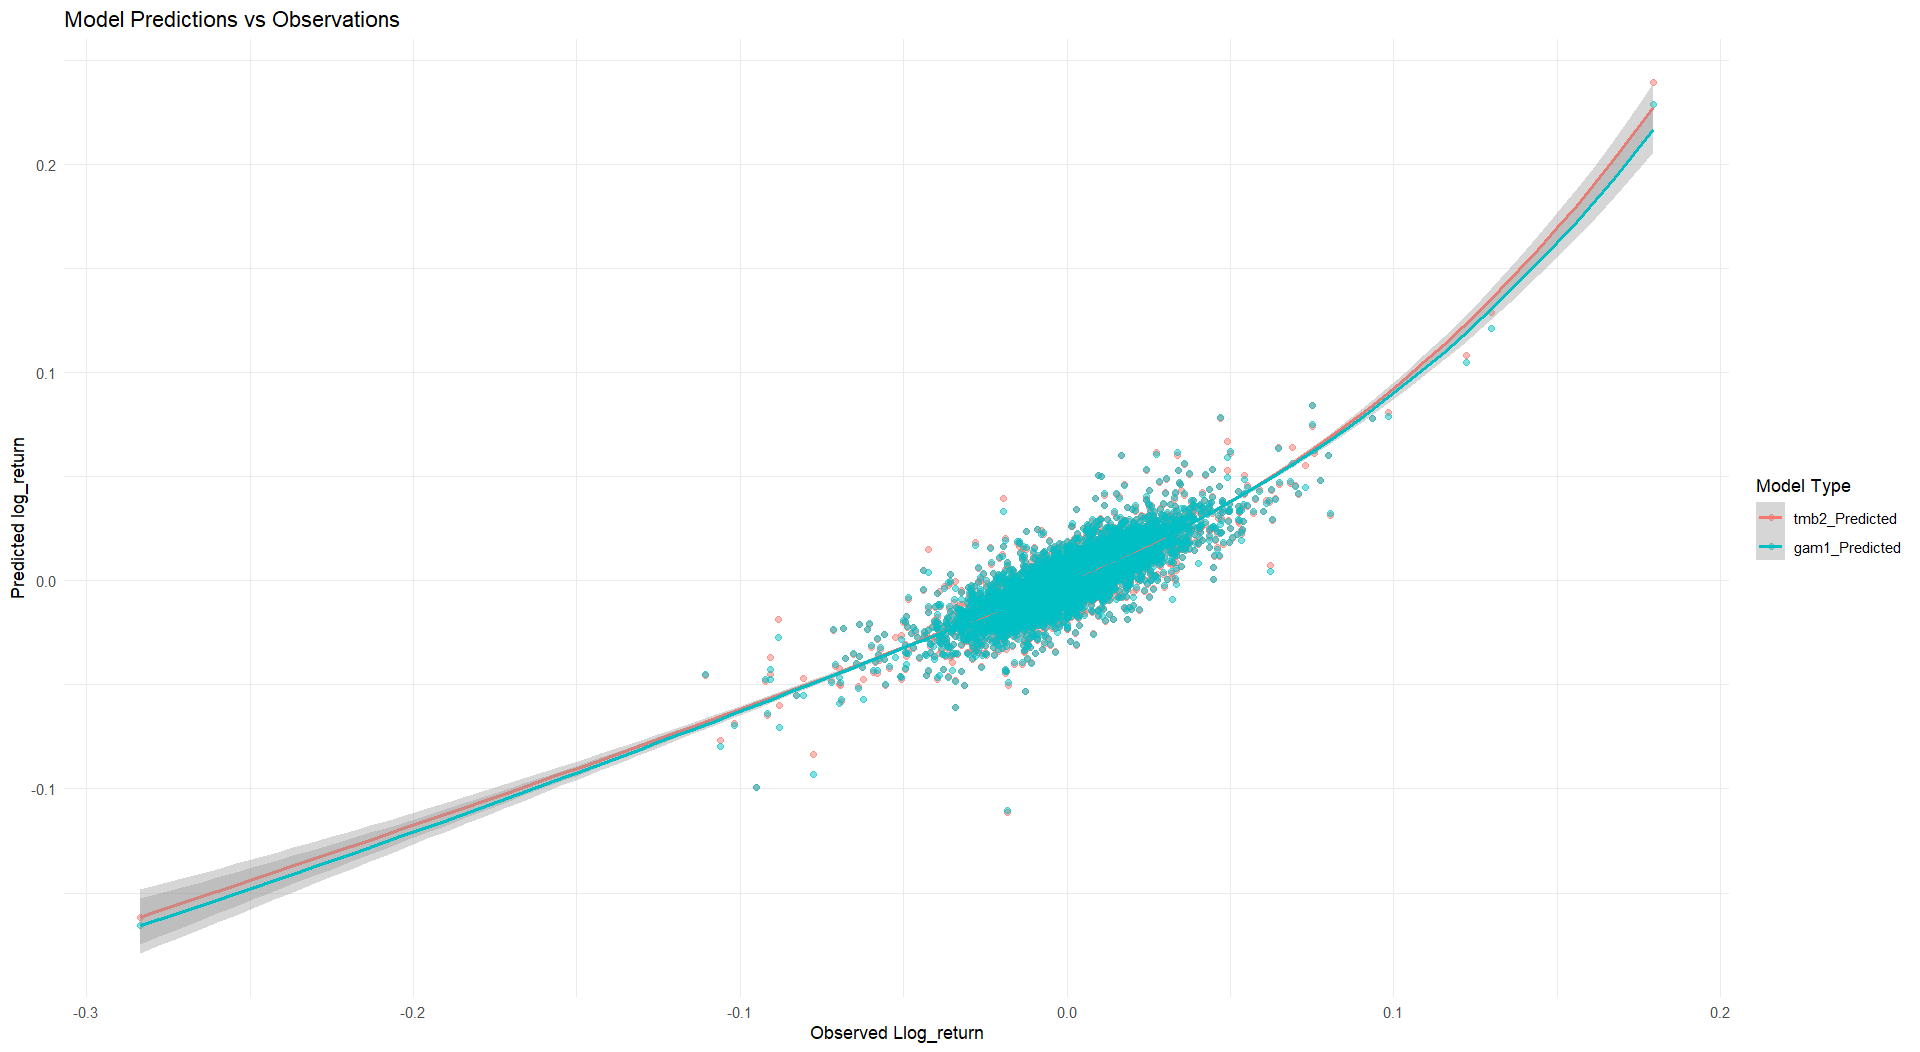
\includegraphics[width=0.9\linewidth]{visuals/pred_obs_snow.png}
    \caption{Prediction vs Observation for SNOW}
\end{figure}




\end{document}



